\section{Zone of Proximal Policy Optimization}
\label{sec:method}

% figure
\begin{figure*}[t!]
    \vspace{-3mm}
    \centering
    
\includegraphics[width=\linewidth]{figures/figure3.pdf}
    \vspace{-5mm}
    \caption{Cumulative graduate counts (graduated\,/\,admitted $=$ ratio) for ZPPO vs.\ GRPO$^{\dagger}$ at 2B by entry rollout accuracy at admission; $^{\dagger}$ denotes augmentation with the prompt replay buffer.}
    \label{fig:zone}
    % \vspace{-5mm}
\end{figure*}

ZPPO is built on top of GRPO~\citep{shao2024deepseekmath}. We first set up notation and identify the precise failure mode that motivates ZPPO (Sec.~\ref{sec:method:prelim}); we then describe the two prompt reformulations BCQ and NCQ that recover a learning signal on hard questions (Sec.~\ref{sec:method:bcqncq}) and the prompt replay buffer that amplifies them (Sec.~\ref{sec:method:buffer}). How the reformulated rollouts plug into the training loop, together with two recipe-level choices on the backbone, is described at Sec.~\ref{sec:experiments:setup}. The full ZPPO training step is summarized as Algorithm~\ref{alg:zppo} in Appendix~\ref{sec:appendix:algorithm}.

\subsection{Preliminaries: GRPO's Failure Mode}
\label{sec:method:prelim}

Let $x$ denote a question and $y_{\rm S}$ a response sampled from a student policy $\pi_\theta$. For each $x$ we draw a group of $G_{\rm S}$ student rollouts $\{y_{\rm S}^{(g)}\}_{g=1}^{G_{\rm S}} \sim \pi_\theta(\cdot \mid x)$ and assign each an outcome reward $r(x, y_{\rm S}^{(g)}) \in \{0, 1\}$ that signals whether the final answer is correct. Let $\bar{r}_x$ and $\mathrm{std}_x$ denote the within-group mean and standard deviation of $\{r(x, y_{\rm S}^{(g)})\}_{g=1}^{G_{\rm S}}$. The standard group-relative advantage~\citep{shao2024deepseekmath,yu2025dapo} is
\begin{equation}
A^{(g)} \;=\; \frac{r(x, y_{\rm S}^{(g)}) - \bar{r}_x}{\mathrm{std}_x + \epsilon}.
\label{eq:grpo-adv}
\end{equation}
Eq.~\eqref{eq:grpo-adv} is the textbook group-relative advantage that ZPPO conceptually builds on; the exact estimator used in our experiments is the two-step REINFORCE++ variant of \citet{hu2025reinforce++} (Step~1 subtracts the per-group mean; Step~2 batch-normalizes across the non-trivial groups), restated in our notation as Eqs.~\eqref{eq:adv-step1}--\eqref{eq:adv-step2} in Appendix~\ref{sec:appendix:algorithm}. The student update applies the PPO surrogate~\citep{schulman2017proximal} on top of $A^{(g)}$. Either form leaves a blind spot for small students. Whenever a rollout group is all-wrong ($\bar{r}_x\!=\!0$) or all-correct ($\bar{r}_x\!=\!1$), every advantage in the group is exactly zero, so the question contributes no gradient signal at all. For a small student, the all-wrong case is exactly the set of questions that could be solved with teacher guidance. ZPPO's goal is to recover a learning signal on those hard questions \emph{without ever placing a teacher response in the student's gradient}. We call $x$ a \emph{hard question} when $\bar{r}_x<0.5$ and use this single threshold throughout; the cutoff is not arbitrary, since under $\{0,1\}$ rewards $\mathrm{std}_x$ is maximized at $\bar{r}_x\!=\!0.5$, where the group-relative advantage carries the strongest learning signal~\citep{liu2025understanding}.

\subsection{Prompt Reformulation: BCQ and NCQ}
\label{sec:method:bcqncq}

Both BCQ and NCQ start from a hard question $x$ on which we have already drawn $G_{\rm S}$ student rollouts $\{y_{\rm S}^{(g)}\}_{g=1}^{G_{\rm S}}$. In parallel, we sample $G_{\rm T}$ teacher rollouts on $x$ from a frozen teacher policy $\pi_{\rm T}$, score them with the same outcome reward, and keep the correct ones as the pool $\{y_{\rm T}^{(+)}\}$ from which BCQ draws candidates. We use \emph{on-policy} throughout in the \emph{response-level} sense: every gradient-counted token is sampled from the current student. BCQ/NCQ prompts do contain teacher-derived text (correct and wrong candidate traces and, for NCQ, the parsed wrong-answer list), but this text is part of the input prompt and never enters the policy gradient as a target. Because we re-sample teacher rollouts every time $x$ is seen -- whether new or replayed from $\mathcal{B}$ -- the candidates that BCQ uses change on every visit.

\textbf{(i) Candidate compression:} Before any candidate enters a prompt, the frozen teacher rewrites it into a short reasoning trace under a shared compression prompt and a shared token cap (Appendix~\ref{sec:appendix:hyperparameters}); the same prompt and cap are applied to teacher-correct and student-wrong traces. The rewritten text still appears only inside the prompt.

\textbf{(ii) Binary Candidate-included Question (BCQ):} For each hard question that admits at least one correct teacher response, BCQ uniformly samples one $y_{\rm T}^{(+)}$ and one wrong student rollout $y_{\rm S}^{(-)}$, teacher-compresses both responses, anonymizes them inside identical \texttt{<candidate>} tags, randomly shuffles the order, and appends the result to $x$ together with a single instruction (the verbatim code-side template, including the per-candidate \texttt{<candidate>} blocks, is reproduced in Appendix~\ref{sec:appendix:hyperparameters:zppo}):
\begin{prompttemplate}
\footnotesize
\emph{Here are two candidate responses in \texttt{<candidate>} \texttt{</candidate>} tags to the question above. One is correct and another is wrong.}
\end{prompttemplate}
The student then samples a new rollout group $\{y_{\rm BCQ}^{(g)}\}_{g=1}^{G_{\rm S}} \sim \pi_\theta(\cdot \mid x_{\rm BCQ})$ from the reformulated prompt; every response token is generated by the current student, so the policy gradient remains on-policy. The pedagogical effect comes from placing a correct teacher response and a wrong student response \emph{side by side} -- anonymized, shuffled, and presented without a correctness label -- so the student is trained to select and reason between the two candidates without any explicitly labeled target entering the gradient.
\begin{figure*}[t!]
    \vspace{-3mm}
    \centering
    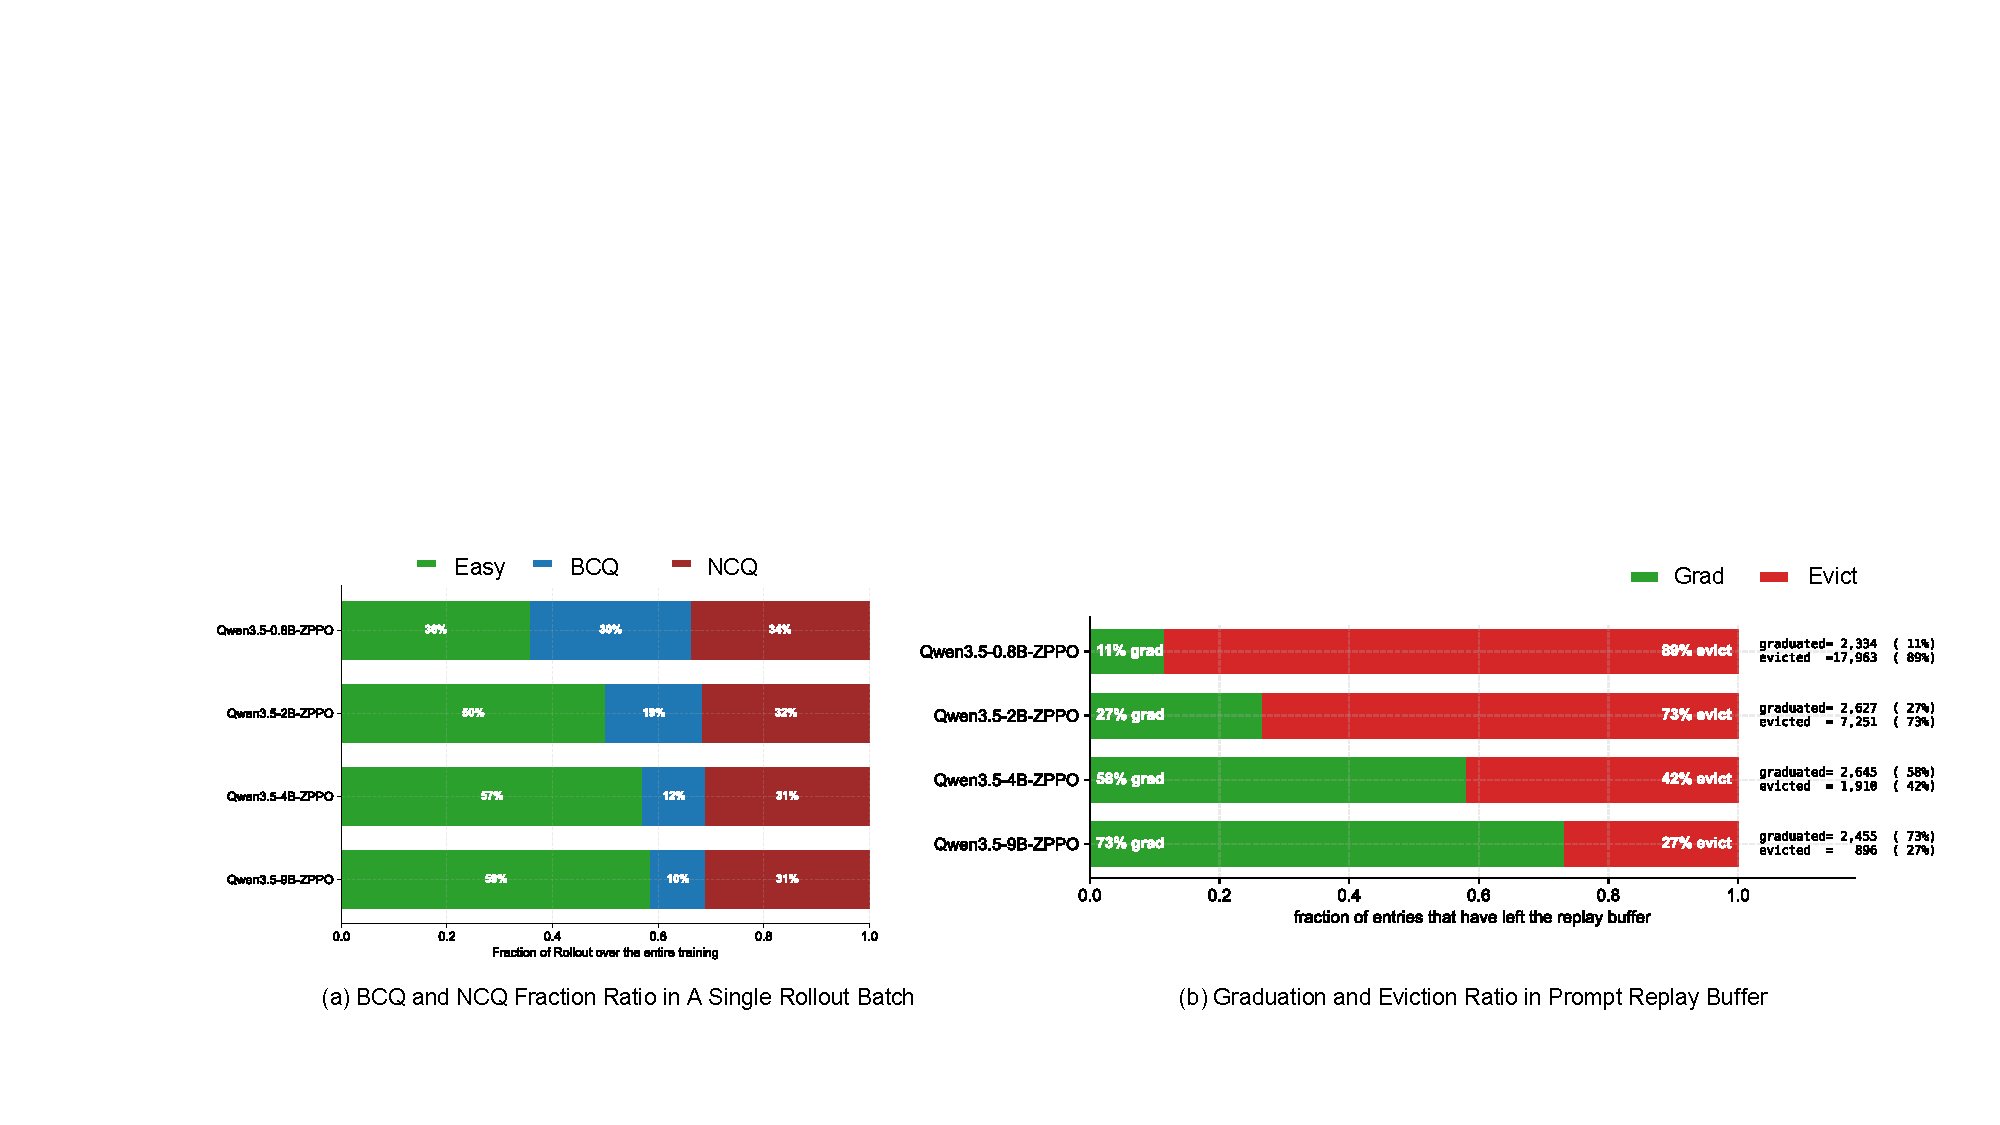
\includegraphics[width=\linewidth]{figures/figure4.pdf}
    \vspace{-5mm}
    \caption{(a)~Composition of a single training rollout batch over the full run into Easy ($\bar{r}_x\!\ge\!0.5$), BCQ, and NCQ shares, per student scale. (b)~Cumulative graduation vs.\ FIFO-eviction ratio of the prompt replay buffer.}
    \label{fig:system}
    % \vspace{-5mm}
\end{figure*}

\textbf{(iii) Negative Candidate-included Question (NCQ):} For each hard question, NCQ collects \emph{every} wrong student rollout $y_{\rm S}^{(-)}$ in the current group, parses out each rollout's final answer and lists the parsed answers explicitly inside the prompt, and appends each teacher-compressed reasoning trace as a \texttt{<candidate>} block, with the instruction (verbatim code-side template in Appendix~\ref{sec:appendix:hyperparameters:zppo}):
\begin{prompttemplate}
\footnotesize
\emph{The following answers are all WRONG: $\langle$\,parsed answer\,$\rangle$. Below are the incorrect reasoning processes in \texttt{<candidate>} \texttt{</candidate>} tags.}
\end{prompttemplate}
The student then samples a new rollout group $\{y_{\rm NCQ}^{(g)}\}_{g=1}^{G_{\rm S}} \sim \pi_\theta(\cdot \mid x_{\rm NCQ})$. As with BCQ, every $y_{\rm NCQ}^{(g)}$ is entirely student-generated, so the policy gradient is on-policy at the response level. The pedagogical role of NCQ, however, is structurally different. In a standard rollout group, each wrong rollout contributes its own advantage to the student's policy gradient independently, and -- within independent rollout groups -- the student has no way to see patterns across its failures. Within our training loop, NCQ is the first place at which independently sampled wrong rollouts on the same question converge into a single prompt: confronted with its own failed attempts, the student is cued to recognize the shared error patterns and avoid them.


\subsection{Integration with Prompt Replay Buffer}
\label{sec:method:buffer}

The prompt replay buffer $\mathcal{B}$ exists \emph{solely to amplify BCQ and NCQ} on questions the student has not yet mastered. It stores only the question $x$ (image and text), never any rollout responses.

\textbf{(i) Admission and graduation:} After each training step we update $\mathcal{B}$ from the current rollout batch: a question $x$ is \emph{admitted} if its $\bar{r}_x\!<\!0.5$, and an already-admitted $x$ is \emph{graduated} (removed) on any later step where $\bar{r}_x$ reaches half ($\bar{r}_x\!\geq\!0.5$). Because BCQ and NCQ are constructed only on hard questions, every replayed question is eligible for one or both reformulations on its next visit. The buffer therefore always tracks the student's \emph{current} zone of proximal development.

\textbf{(ii) Sampling and capacity:}
Each rollout batch combines new questions from the data loader with replay samples drawn uniformly from $\mathcal{B}$, where the replay count is a fixed fraction $\rho_{\rm replay}$ of the new-question count. From the union of new and replayed questions, BCQ and NCQ are constructed on the hardest ones first (ranked by ascending $\bar{r}_x$); the \emph{combined} BCQ+NCQ count per rollout step is then capped at a fraction $\rho_{\rm aug}$ of the new-question count (Appendix~\ref{sec:appendix:algorithm}). The buffer therefore re-exposes each hard question many times -- with freshly sampled BCQ/NCQ candidates on every visit -- until it either graduates or is FIFO-evicted once $|\mathcal{B}|$ exceeds $|\mathcal{B}|_{\max}$. (see Appendix~\ref{sec:appendix:algorithm} for ZPPO algorithm)